\section{AstroLoc Library Overview}
The AstroLoc library offers useful tools for localization, odometry, calibration, mapping, and more using GTSAM graph-based optimization.
The library consists of graph optimizer and sliding window graph optimizer classes that use node adders and factor adders for node and factor creation, where nodes are state parameters optimized in the graph.
\begin{figure}[ht]
    \centering
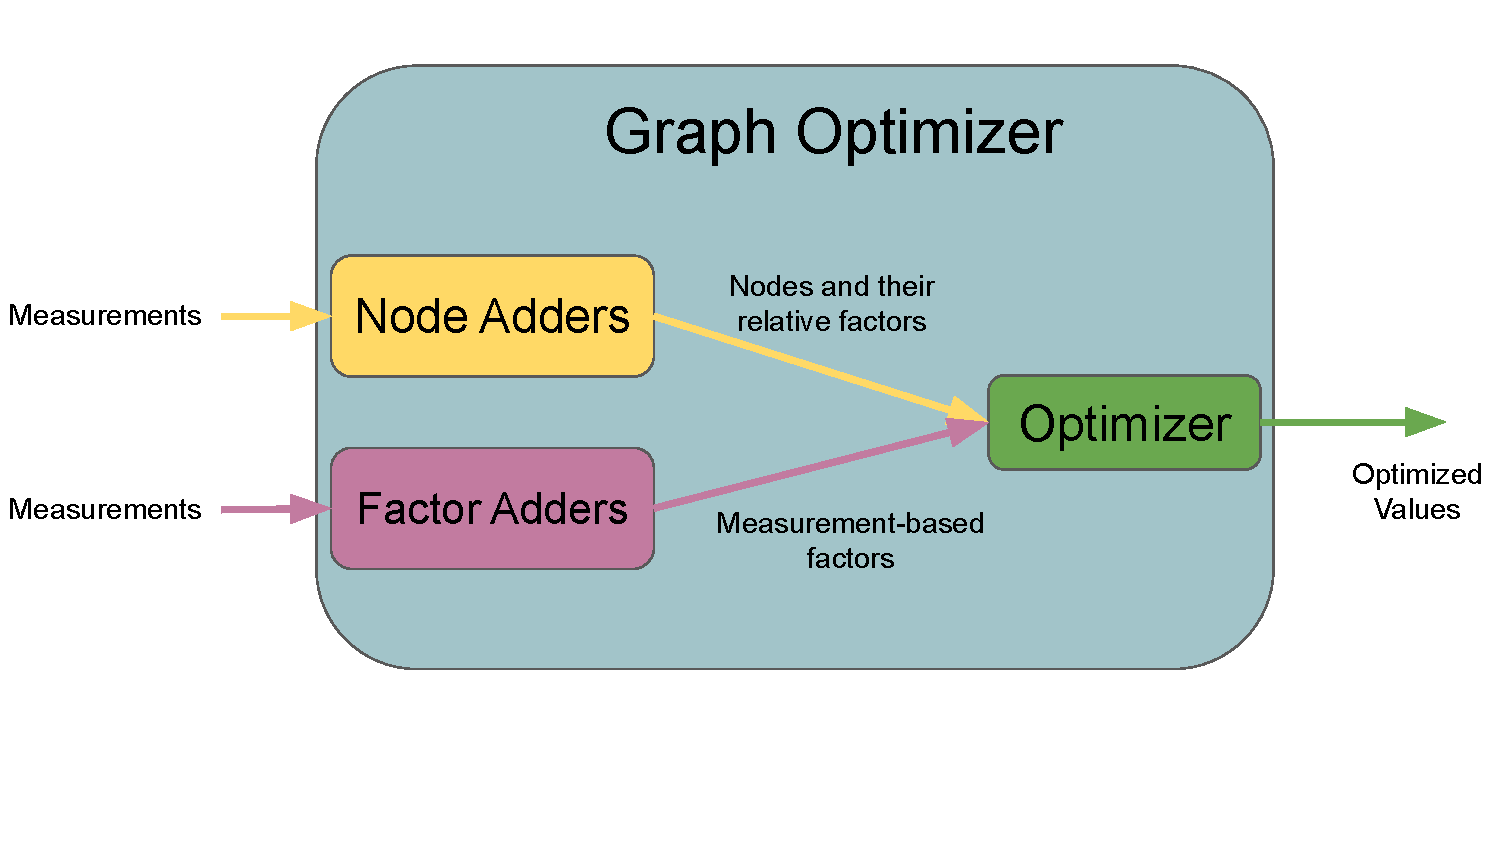
\includegraphics[width=0.9\textwidth]{graph_opt.pdf}
 \caption{A graph optimizer contains node adders that create nodes and relative factors connecting them and factor adders that create measurement-based factors for certain nodes in the graph.}
  \label{img:graph_opt}
\end{figure}
The library contains packages for each of these objects and has useful factor and node adders already implemented to help perform localization, odometry, calibration, and mapping. 
\subsection{Optimizers}\label{sec:overview}
Nonlinear and ISAM2 optimizers can be used for graph optimization.
ISAM2 \cite{kaess2012isam2} is particularly helpful for mapping when keeping a large history of nodes to optimize, whereas often nonlinear optimization is sufficient for performing sliding window optimization.
\subsection{Graph Optimizer and Sliding Window Graph Optimizer}
\subsubsection{Graph Optimizer}
The graph optimizer shown in Figure ~\ref{img:graph_opt} contains a GTSAM factor graph and factor and node adders that process input measurements and output the nodes and factors used for optimization.
It contains functions to perform optimization and access covariances for its nodes.
\subsubsection{Sliding Window Graph Optimizer}
The sliding window graph optimizer in Figure ~\ref{img:sliding_window_graph_opt} extends the graph optimizer for sliding window optimization and uses sliding window node adders that remove old nodes and factors that fall outside of the window. 
It uses an Update() function call that adds factors from factor adders up to the latest measurements, optimizes the graph, and slides the window as required.
The sliding window size is defined in both a maximum duration and number of nodes and is configured in the sliding window parameters.
\begin{figure}[ht]
    \centering
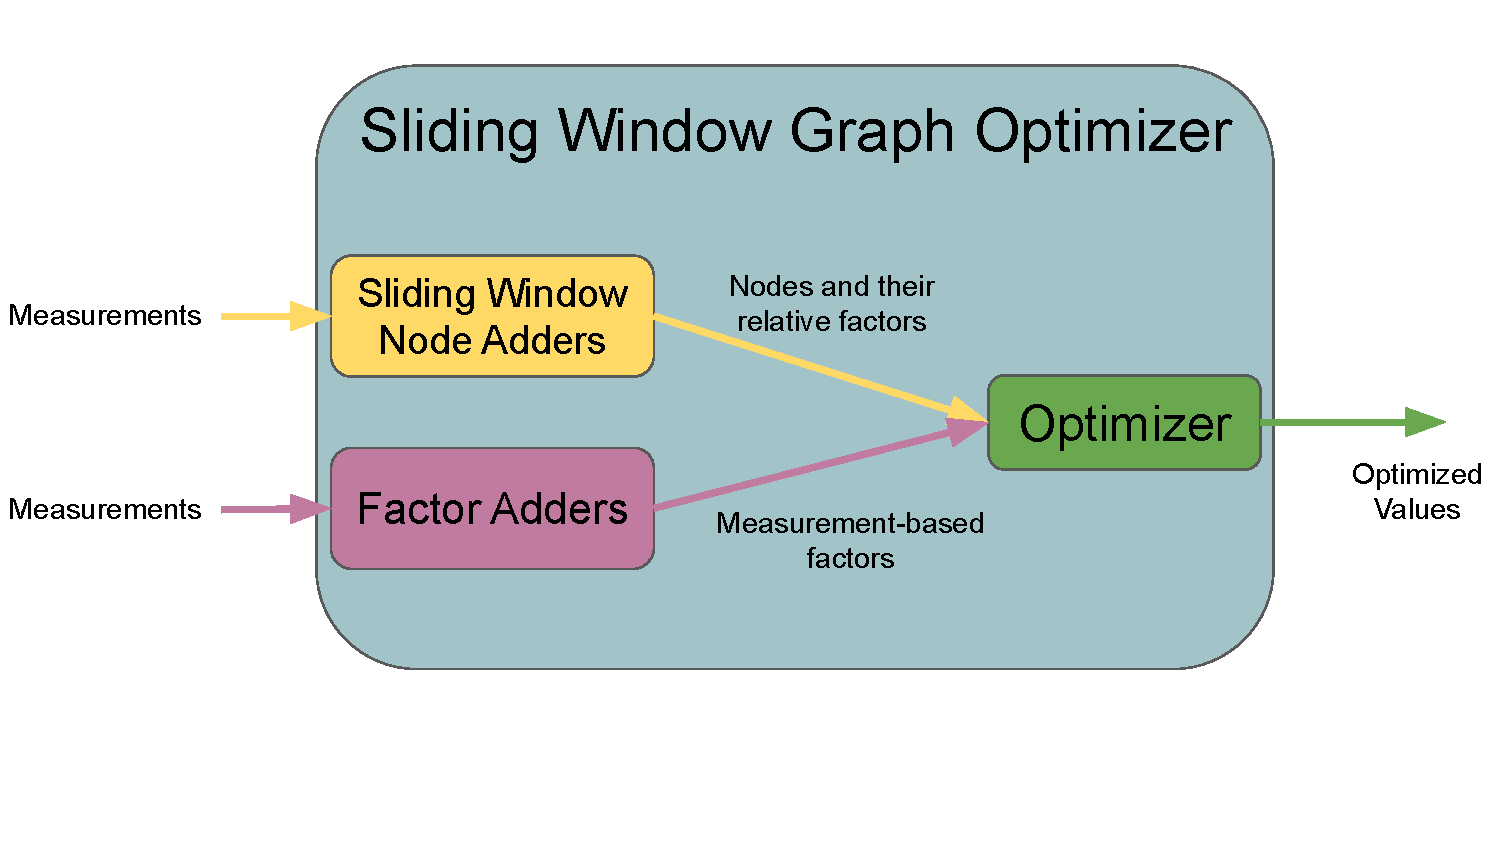
\includegraphics[width=0.9\textwidth]{sliding_window_graph_opt.pdf}
 \caption{The sliding window graph optimizer uses sliding window node adders that remove old nodes and factors as required.}
  \label{img:sliding_window_graph_opt}
\end{figure}
\subsection{Node Adders}
The node adders displayed in Figure ~\ref{img:node_adder} define the node type to be optimized and are in charge of adding relative factors and nodes to the graph for those types.
A node adder is templated on measurement, node, timestamped nodes, and node adder model types.
\begin{figure}[H]
    \centering
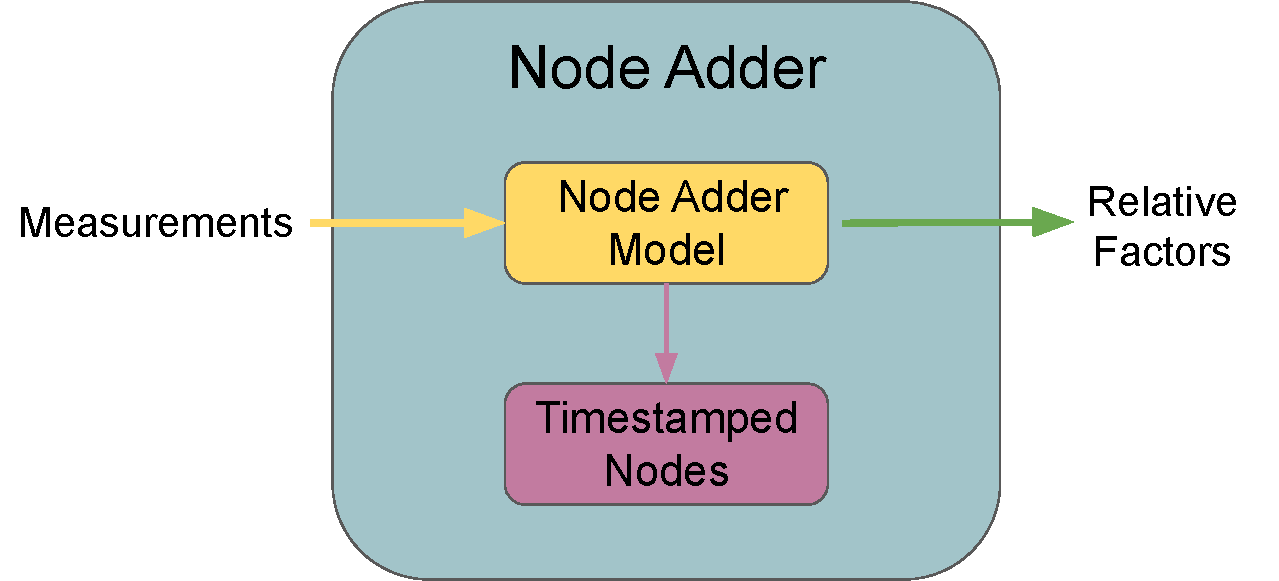
\includegraphics[width=0.9\textwidth]{node_adder.pdf}
 \caption{A node adder taking measurements and using a node adder model to generate timestamped nodes and relative factors.}
  \label{img:node_adder}
\end{figure}
\subsubsection{Measurement Type}
The measurement is passed to the node adder model and contains the information necessary to create future nodes and relative factors.
\subsubsection{Node and TimestampedNodes Types}
The node type specifies the state parameter optimized in the graph optimizer.
The timestamped nodes type specifies the container for interfacing with the nodes in the optimizer.
For simple, single-typed timestamped values, such as a pose or point, the TimestampedNodes class should be used.
For nodes containing multiple types (i.e. a pose, velocity, and bias for VIO), use the TimestampedCombinedNodes class and make sure to override the required functions for adding and accessing nodes.
See CombinedNavStateNodes in the nodes package for an example.
Multiple node adders can exist in a single graph optimizer that handle different node types, and all these are optimized together in the same graph.
\subsubsection{Node Adder Models}
The node adder model handles adding nodes and relative factors and stores measurements used for creating these. 
Prefer using the BetweenFactorMeasurementBasedTimestampedNodeAdderModel class which adds relative factors using gtsam::BetweenFactors for a single-valued node type.
For more complicated relative factors, use MeasurementBasedTimestampedNodeAdderModel and customize the functions for adding relative nodes and factors as desired.
See the CombinedNavStateNodeAdder in the node adders package for an example.
\subsection{Factor Adders}
The factor adders illustrated in Figure ~\ref{img:factor_adder} add measurement-based factors that can depend on single or multiple node values.
For factor creation that depends on a single measurement at a time, use SingleMeasurementBasedFactorAdder, otherwise use MeasurementBasedFactorAdder.
\begin{figure}[h]
    \centering
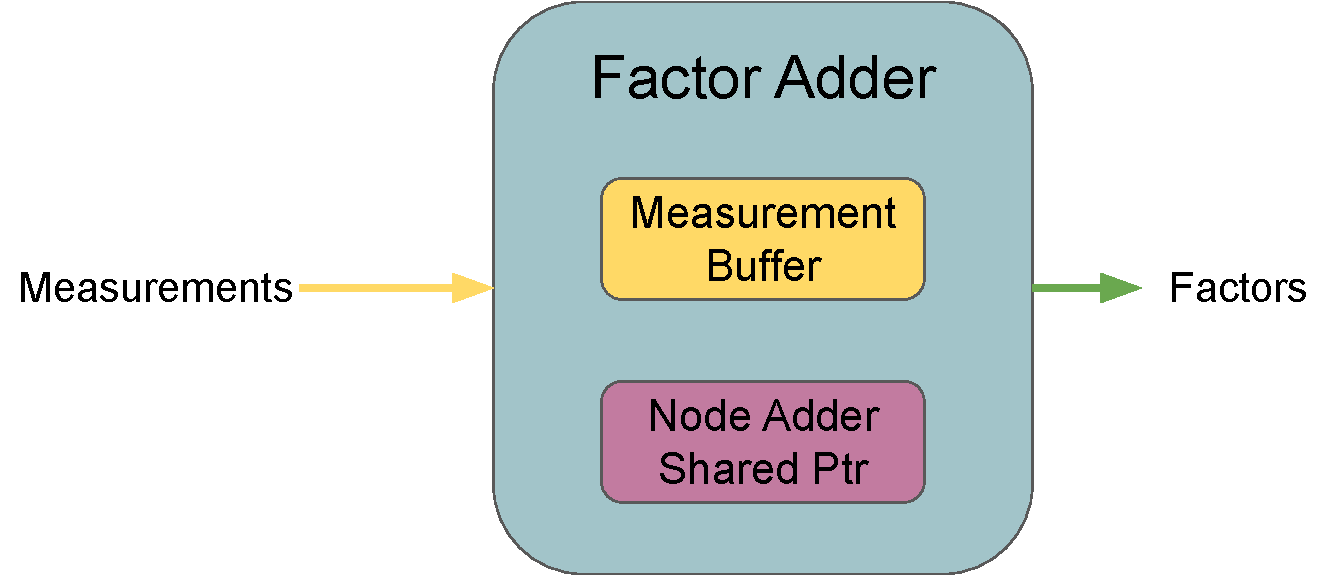
\includegraphics[width=0.9\textwidth]{factor_adder.pdf}
 \caption{A factor adder taking measurements and generating factors. Nodes are created for the graph at the measurement timestamp using a shared node adder.}
  \label{img:factor_adder}
\end{figure}